\let\negmedspace\undefined
\let\negthickspace\undefined
\documentclass[journal,12pt,onecolumn]{IEEEtran}
\usepackage{cite}
\usepackage{amsmath,amssymb,amsfonts,amsthm}
\usepackage{algorithmic}
\usepackage{graphicx}
\graphicspath{{./figs/}}
\usepackage{textcomp}
\usepackage{xcolor}
\usepackage{txfonts}
\usepackage{listings}
\usepackage{enumitem}
\usepackage{mathtools}
\usepackage{gensymb}
\usepackage{comment}
\usepackage{caption}
\usepackage[breaklinks=true]{hyperref}
\usepackage{tkz-euclide} 
\usepackage{listings}
\usepackage{gvv}                                        
%\def\inputGnumericTable{}                                 
\usepackage[latin1]{inputenc}     
\usepackage{xparse}
\usepackage{color}                                            
\usepackage{array}
\usepackage{longtable}                                       
\usepackage{calc}                                             
\usepackage{multirow}
\usepackage{multicol}
\usepackage{hhline}                                           
\usepackage{ifthen}                                           
\usepackage{lscape}
\usepackage{tabularx}
\usepackage{array}
\usepackage{float}
\newtheorem{theorem}{Theorem}[section]
\newtheorem{problem}{Problem}
\newtheorem{proposition}{Proposition}[section]
\newtheorem{lemma}{Lemma}[section]
\newtheorem{corollary}[theorem]{Corollary}
\newtheorem{example}{Example}[section]
\newtheorem{definition}[problem]{Definition}
\newcommand{\BEQA}{\begin{eqnarray}}
\newcommand{\EEQA}{\end{eqnarray}}
\newcommand{\define}{\stackrel{\triangle}{=}}
\theoremstyle{remark}
\newtheorem{rem}{Remark}

\begin{document}

\title{9.6.5}
\author{ee25btech11056 - Suraj.N}
\maketitle
\renewcommand{\thefigure}{\theenumi}
\renewcommand{\thetable}{\theenumi}

\begin{document}

\textbf{Question :} Solve
\[
\frac{1}{3x+y} + \frac{1}{3x-y} = \frac{3}{4}, \quad 
\frac{1}{2(3x+y)} - \frac{1}{2(3x-y)} = -\frac{1}{8}.
\]

\textbf{Solution :}

\begin{table}[h!]
  \centering
  \begin{tabular}{|c|c|}
\hline
\textbf{Name} & \textbf{Value} \\ \hline
$\vec{A}$ & $\myvec{2 & 1 \\0 & 3}$ \\ \hline
\end{tabular}

  \caption*{Table : Hyperbola}
  \label{9.6.5}
\end{table}

By rearranging the two equations we get the equation of two hyperbolas as :

\begin{align}
  9x^2 - y^2 -8y &= 0\\
  9x^2 - y^2 -8x &= 0
\end{align}

The conic parameters for the two hyperbolas can be expressed as :

\begin{align}
  \vec{V_1} &= \myvec{9 & 0\\0 & -1} & \vec{u_1} &= \myvec{0 \\ -4} & f1 &= 0\\
  \vec{V_2} &= \myvec{9 & 0\\0 & -1} & \vec{u_2} &= \myvec{-4 \\ 0} & f2 &= 0
\end{align}

The intersection of two conics is defined as :

\begin{align}
  \vec{x}^\top(\vec{V_1}+\mu\vec{V_2})\vec{x} + 2(\vec{u_1}+\mu\vec{u_2})^\top\vec{x} + (f1 + \mu f2) = 0 \label{eq:conic} 
\end{align}

The above equation represents a pair of straight lines if :

\begin{align}
  \mydet{\vec{V_1}+\mu\vec{V_2} & \vec{u_1}+\mu\vec{u_2}\\(\vec{u_1}+\mu\vec{u_2})^\top & f1 + \mu f2} &= 0
\end{align}

Substituting the values in the above equation :

\begin{align}
  \mydet{9+9\mu & 0 & -4\mu\\0 & -1-\mu & -4\\-4\mu & -4 & 0} &= 0
\end{align}

Applyint row reduction to find determinant:

\begin{align}
\mydet{9+9\mu & 0 & -4\mu\\0 & -1-\mu & -4\\-4\mu & -4 & 0} 
\xleftrightarrow{R_3 \to R_3 +\tfrac{4\mu}{9+9\mu}R_1}
\mydet{9+9\mu & 0 & -4\mu\\0 & -1-\mu & -4\\0 & -4 & -\tfrac{16\mu^2}{9+9\mu}}
\xleftrightarrow{R_3 \to R_3 -\tfrac{4}{1+\mu}R_2}
\mydet{9+9\mu & 0 & -4\mu\\0 & -1-\mu & -4\\0 & 0 & \tfrac{-16\mu^2+144}{9+9\mu}}
\end{align}

\pagebreak

By finding the determinant we get 

\begin{align}
  (1+\mu)(-16\mu^2 + 144) &= 0\\
  \mu = -1 , \mu = \pm3
\end{align}

Substituting $\mu = -1$ in \eqref{eq:conic} we get equation of line as :

\begin{align}
  2\myvec{4 \\-4}^\top\vec{x} &= 0\\
  \myvec{-1 & 1}\vec{x} &= 0
\end{align}

The parameters of the line are :

\begin{align}
  \vec{h} &= \myvec{0\\0} & \vec{m} &= \myvec{1\\1}
\end{align}

Substituting the parameters of line and the first hyperbola in the below equation :

\begin{align}
\kappa_i
  &= \frac{1}{\vec{m}^\top \vec{V_1}\vec{m}}
     \left(
       -\,\vec{m}^\top\big(\vec{V_1}\vec{h}+\vec{u_1}\big)
       \;\pm\;
       \sqrt{ \big[\vec{m}^\top(\vec{V_1}\vec{h}+\vec{u_1})\big]^2
       - g(\vec{h})\,\big(\vec{m}^\top \vec{V_1}\vec{m}\big)}
     \right)\\
  \kappa_i &= 0,1
\end{align}

Therefore the points of intersections of the line and first hyperbola are :

\begin{align}
  \vec{P_1}&=\myvec{1\\1} & \vec{P_2} = \myvec{0\\0}
\end{align}

But if we substiture $\vec{P_2}$ in the original equation we get 0 in the denominator , which is undefined.\\
Therefore the solution for the given equations is :

\begin{align}
  \vec{P} &= \myvec{1\\1}
\end{align}


\pagebreak

\begin{figure}[h!]
  \centering
  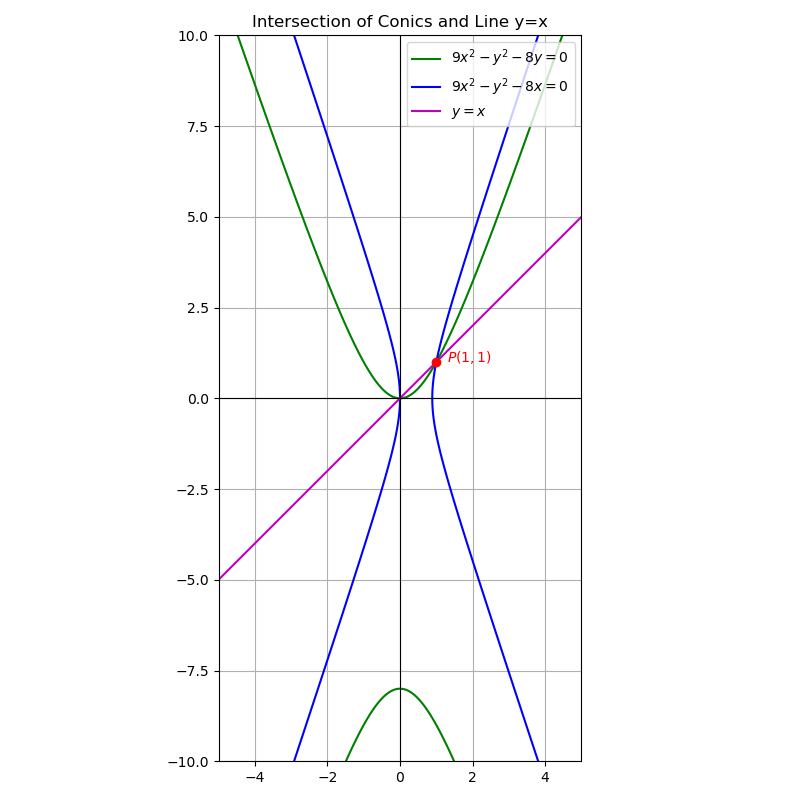
\includegraphics[width=0.7\columnwidth]{figs/conics_intersection.png} 
   \caption*{Fig : Hyperbola and Line}
  \label{Fig1}
\end{figure}

\end{document}
